\chapter{Modélisation des actions entre solides}
	\section{Torseur des actions mécaniques}
		\subsection{Définition}
					
\begin{wrapfigure}{l}{0.4\textwidth}
	\centering
	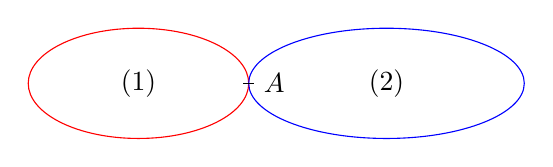
\begin{tikzpicture}[scale=0.7]
		\draw[red] (0,0) ellipse (2 and 1);
		\node at (0,0) {$(1)$};
		\draw[blue] (4.5,0) ellipse (2.5 and 1);
		\node at (4.5,0) {$(2)$};
		\draw (2,0) -- ++(0.1,0) node[anchor=west]{$A$};
		\draw (2,0) -- ++(-0.1,0);
	\end{tikzpicture}
\end{wrapfigure}
Soient deux solides $(1)$ et $(2)$, en contact mutuel en $A$. L'action de $(1)$ sur $(2)$ est représenté par le torseur des actions mécaniques suivant :
\medskip
\hidden{
\begin{equation}
	\torseur{F}{1\rightarrow2}=\left\lbrace
		\begin{array}{c}
				\R{1}{2}\\
				\M{A}{1}{2}
		\end{array}
	\right\rbrace_A
\end{equation}
}

$\R{1}{2}$ est la force appliquée par $(1)$ sur $(2)$ tandis que $\M{A}{1}{2}$ est le moment en $A$ de l'effort appliqué par $(1)$ sur $(2)$.

		\subsection{Cas particuliers}
		\begin{itemize}
			\item Si la résultante des efforts de $(1)$ sur $(2)$ est nulle, alors on dit que l'action de $(1)$ sur $(2)$ est un couple pur. Ce couple est constant, d'après la formule du champ de moments de torseur.
			\item Si le moment est nul en un point $A$, alors le torseur est un \emph{glisseur}.
		\end{itemize}
		
		\section{Champ de pesanteur}
		\label{sec:centre-de-masse}
		\subsection{Centre d'inertie}
\begin{definition}
\hidden{
Soit $G$ un point d'un solide $S$. $G$ est d'inertie de $S$ si et seulement si :
	\begin{equation}
		\int_{P\in S}\vect{GP}\dm=\vect{0}
		\label{eq:def-G}
	\end{equation}
}
\end{definition}

\begin{theorem}
\hidden{
	Soit un solide $S$ de masse $m$. Le centre d'inertie $G$ de $S$ vérifie alors :
	\begin{equation}
		\forall A\quad\vect{AG}=\frac{1}{m}\int_{P\in S}\vect{AP}\dm
	\end{equation}	 
}
\end{theorem}

\begin{proof}
	\begin{alignat*}{7}
		&&&\vect{AP}&&=&&\vect{AG}&&+&&\vect{GP}&\\
		&\implies\quad& \int_{P\in S}&\vect{AP}&\dm&=&\int_{P\in S}&\vect{AG}&\dm&+&\int_{P\in S}&\vect{GP}&\dm\\
		&\iff\quad& \int_{P\in S}&\vect{AP}&\dm&=&&\vect{AG}&\int_{P\in S}\dm&+&&\vect{0}&\\
		&\iff\quad& \int_{P\in S}&\vect{AP}&\dm&=&&\vect{AG}m&
	\end{alignat*}
\end{proof}

		\subsection{Actions du champ de pesanteur}

\begin{theorem}
\hidden{
	Soit $S$ un solide de masse $m$ soumis au champ de pesanteur, supposé uniforme et dirigé suivant une direction $-\vect{z}$ : $\vect{g}=-g\vect{z}$. Le torseur des actions de pesanteur s'écrit alors :
	\begin{equation}
		\torseur{F}{g\rightarrow S}=\left\lbrace
			\begin{array}{c}
					-mg\vect{z}\\
					\vect{0}
			\end{array}
		\right\rbrace_G
	\end{equation}
}	
\end{theorem}

\begin{proof}
	Soit un petit élément de masse $\dm$ de $S$. L'action de pesanteur sur cet élément vaut alors :
	\begin{alignat*}{4}
		&&				&\mathrm{d}\R{g}{S}	&=&-\vect{g} \dm&\\
		&\implies\quad&	&\R{g}{S}			&=&\int_{P\in S}\vect{g}\dm&=\int_{P\in S}-g\vect{z}\dm=-g\vect{z}\int_{P\in S}\dm\\
		&\iff\quad&&\R{g}{S}&=&-mg\vect{z}&
	\end{alignat*}
	
	De la même façon, si on calcule le moment en $A$ :
	\begin{equation*}
		\M{A}{g}{S}=\int_{P\in S}\vect{AP}\wedge\left(-g\vect{z}\right)\dm
		=-g\int_{P\in S}\vect{AP}\wedge\vect{z}\dm
		=-g\left(\int_{P\in S}\vect{AP}\dm\right)\wedge\vect{z}
	\end{equation*}
	
Soit $G$ le centre de gravité de $S$. On a alors~\eqref{eq:def-G} :
\begin{equation*}
	\int_{P\in S}\vect{GP}\dm=\vect{0}
\end{equation*}
On a alors :
\begin{equation*}
	\M{G}{g}{S}=\vect{0}
\end{equation*}	
\end{proof}

\section{Actions de contact}
	\subsection{Contact ponctuel}
	\begin{minipage}[b]{0.4\textwidth}
		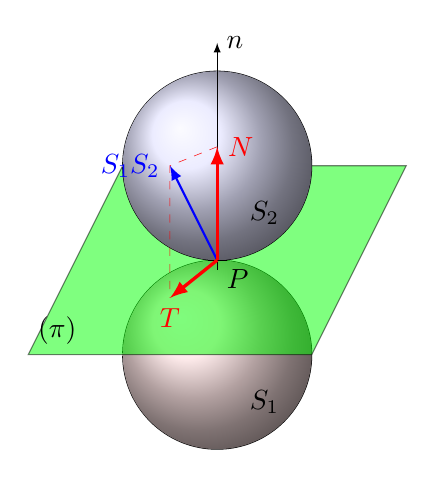
\begin{tikzpicture}[scale=1.2]
		    \draw (0,0) circle (1cm);
		    \shade[ball color=red!10!white] (0,0) circle (1);
		    \draw[fill=green,opacity=0.5] (-1,2) --++ (-1,-2) node[opacity=1,anchor=south west]{$(\pi)$} --++ (3,0) --++ (+1,+2) -- cycle;
		    \draw (0,2) circle (1cm);
		    \shade[ball color=blue!10!white] (0,2) circle (1);
		    \coordinate (P) at (0,1);
		    \draw (P)--++(0.1,0);
		    \draw (P)--++(-0.1,0);
		    \draw (P)--++(0,0.1);
		    \draw (P)--++(0,-0.1);
		    \node[anchor=north west] at (P){$P$};		
			\node at (0.5,-0.5){$S_1$};    
			\node at (0.5,1.5){$S_2$};
			\draw[-latex,very thin] (P)-- ++ (0,2.3) node[anchor=west]{$\vect{n}$}; 
			\coordinate (Om) at (-0.5,2);
			\coordinate (Pn) at (0,2.2);
			\coordinate (Pp) at (-0.5,0.6);
			\draw[blue,thick,-latex] (P) --(Om) node[anchor=east]{$\R{S_1}{S_2}$};
			\draw[red,very thick,-latex] (P) --(Pn) node[anchor=west]{$\vect{N}$};
			\draw[red,very thick,-latex] (P) --(Pp) node[anchor=north]{$\vect{T}$};
			\draw[very thin, dashed,red] (Pn) -- (Om) -- (Pp);
		\end{tikzpicture}
	\end{minipage}
	\begin{minipage}[b]{0.5\textwidth}
		\begin{theorem}
			Soient deux solides $S_1$ et $S_2$, en contact ponctuel en un point $P$. On note $(\pi)$ le plan tangent à $S_1$ et $S_2$ en $P$. L'action qu'exerce $S_1$ sur $S_2$ peut alors être représentée un glisseur, d'axe central passant par $P$ :
			\begin{equation}
				\tf{S_1}{S_2}=
				\begin{tors}{P}
					\R{S_1}{S_2}\\
					\vect{0}
				\end{tors}					
			\end{equation}
		\end{theorem}
	\end{minipage}
	
		On décompose la résultante comme la somme d'un composante normale à $(\pi)$, notée $\vect{N}$ et d'un composante tangentielle, notée $\vect{T}$ :
		\begin{equation}
			\R{S_1}{S_2}=\vect{N}+\vect{T}
		\end{equation}	
 Si on note $\vect{n}$ la normale à  $(\pi)$, on a donc :
		\begin{subequations}
			\begin{align}
				\vect{N} &\parallel \vect{n}\\
				\vect{T} &\perp \vect{n}
			\end{align}
		\end{subequations}
		
	\subsection{Lois de Coulomb}
		\subsubsection{Glissement}
		\begin{minipage}[b]{0.4\textwidth}
			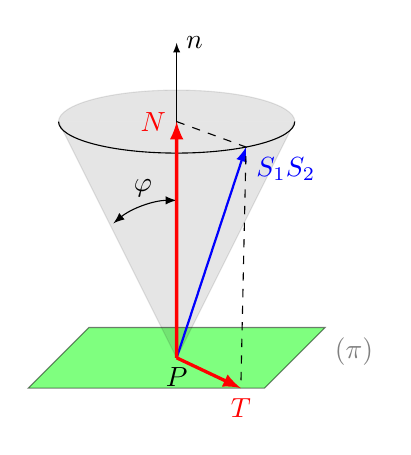
\begin{tikzpicture}
				\coordinate (s) at (-1.5cm,0);
				\draw[-latex,very thin] (s)-- ++ (0,4) node[anchor=west]{$\vect{n}$} coordinate[pos=0.5] (t);
				\draw[fill=green,opacity=0.5] (-3,0,-1) --++ (3,0,0) node[anchor=north west]{$(\pi)$} --++ (0,0,2) --++ (-3,0,0) -- cycle;
				\fill[opacity=0.1,draw] (0,3) arc (0:180:1.5cm and 0.4cm)coordinate[pos=0] (a);
				\draw (0,3) arc (0:-180:1.5cm and 0.4cm)coordinate (b) coordinate[pos=0.3](P);
				\fill[opacity=0.1,draw] (a) -- (s) -- (b);
				\draw[blue,thick,-latex] (s) -- (P) node[anchor=north west]{$\R{S_1}{S_2}$};
				\node[anchor=north] at (s) {$P$};
				\draw[latex-latex] (t) arc (90:130:1.25) node[midway,anchor=south]{$\varphi$};
				\coordinate (pt) at (-0.3,0,1);
				\coordinate (pn) at (-1.5,3);
				\draw[red,very thick,-latex] (s) --(pt) node[anchor=north]{$\vect{T}$};
				\draw[red,very thick,-latex] (s) --(pn) node[anchor=east]{$\vect{N}$};
				\draw[dashed] (pn) -- (P) -- (pt);
  			\end{tikzpicture}
  		\end{minipage}
		\begin{minipage}[b]{0.5\textwidth}
			\begin{theorem}
				Si les solides $S_1$ et $S_2$ glissent l'un sur l'autre, c'est-à-dire si $\V[S_1]{P}{S_2}\neq\vect{0}$ (cf. \S\ref{sec:glissement} p.\pageref{sec:glissement}), on a alors :
				\begin{equation}
					\lVert \vect{T}\rVert=\mu_{\mathrm{d}}\lVert \vect{N}\rVert
				\end{equation}
				et $\vect{T}$ qui est opposé à la vitesse de glissement $\V[S_1]{P}{S_2}$. $\mu_{\mathrm{d}}$ est le coefficient de frottement dynamique.
			\end{theorem}
			\begin{definition}
				On appelle angle de frottement l'angle $\varphi$ tel que :
				\begin{equation}
					\mu_{\mathrm{d}}=\tan\varphi
				\end{equation}
			\end{definition}
			Lors du glissement, la résultante de l'effort est sur le cône de frottement.
		\end{minipage}
		
	\subsubsection{Adhérence}
		\begin{minipage}[b]{0.4\textwidth}
			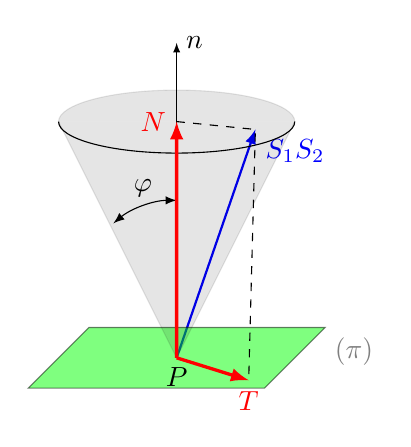
\begin{tikzpicture}
				\coordinate (s) at (-1.5cm,0);
				\coordinate (P) at (-0.5,2.9);
				\draw[blue,thick,-latex] (s) -- (P) node[anchor=north west]{$\R{S_1}{S_2}$};
				\draw[-latex,very thin] (s)-- ++ (0,4) node[anchor=west]{$\vect{n}$} coordinate[pos=0.5] (t);
				\draw[fill=green,opacity=0.5] (-3,0,-1) --++ (3,0,0) node[anchor=north west]{$(\pi)$} --++ (0,0,2) --++ (-3,0,0) -- cycle;
				\fill[opacity=0.1,draw] (0,3) arc (0:180:1.5cm and 0.4cm)coordinate[pos=0] (a);
				\draw (0,3) arc (0:-180:1.5cm and 0.4cm)coordinate (b);
				\fill[opacity=0.1,draw] (a) -- (s) -- (b);
				\node[anchor=north] at (s) {$P$};
				\draw[latex-latex] (t) arc (90:130:1.25) node[midway,anchor=south]{$\varphi$};
				\coordinate (pt) at (-0.2,0.1,1);
				\coordinate (pn) at (-1.5,3);
				\draw[red,very thick,-latex] (s) --(pt) node[anchor=north]{$\vect{T}$};
				\draw[red,very thick,-latex] (s) --(pn) node[anchor=east]{$\vect{N}$};
				\draw[dashed] (pn) -- (P) -- (pt);
  			\end{tikzpicture}
  		\end{minipage}
  		\begin{minipage}[b]{0.5\textwidth}
			\begin{theorem}
				Si les solides $S_1$ et $S_2$ ne glissent pas l'un sur l'autre, c'est-à-dire si $\V[S_1]{P}{S_2}=\vect{0}$, on a alors :
				\begin{equation}
					\lVert \vect{T}\rVert<\mu_{\mathrm{s}}\lVert \vect{N}\rVert
				\end{equation}
				avec $\mu_{\mathrm{s}}$ le coefficient de frottement statique.
			\end{theorem}
			Il y a adhérence si la résultante de l'effort est à l'intérieur du cône de frottement.
		\end{minipage}
		
		Généralement, le coefficient de frottement dynamique est plus faible que le coefficient de frottement statique :
		\begin{equation}
			\mu_{\mathrm{d}}\leq\mu_{\mathrm{s}}
		\end{equation}
